%%%%%%%%%%%%%%%%%%%%%%%%%%%%%%%%%%%%%%%%%%%%%%%%%%%%%%%%%%%%%%%%%%
%%This presentation is a merge of :
%  presentation of the model in JIPI
%% and presentation ABC TRACT 2018

\documentclass[10pt, notes=show]{beamer}
\usetheme[width=0cm]{Goettingen}
\usecolortheme{rose}
\useoutertheme{default}
\setbeamerfont{caption}{size=\scriptsize}
\setbeamertemplate{navigation symbols}{}
\definecolor{tracblue}{RGB}{4,30,67}
\setbeamercolor{title}{fg=tracblue}
\setbeamercolor{frametitle}{fg=tracblue}
\setbeamercolor{structure}{fg=tracblue}

\addtobeamertemplate{navigation symbols}{}{%
    \usebeamerfont{footline}%
    \usebeamercolor[fg]{footline}%
    \hspace{1em}%
    $\dfrac{\insertframenumber}{\inserttotalframenumber}$
}

\usepackage{fontspec} 
\setsansfont{Futura LT}
%\setmonofont[Scale=0.8]{Monaco} 




%\usepackage{amsmath}
%
%\usepackage{mathptmx}
%\usepackage{latexsym}
\usepackage{graphicx}
\usepackage{mathtools}
%\usepackage{media9}
\usepackage{multimedia}
%\usepackage{multirow}
%\usepackage{caption}
%\usepackage{array}
%\usepackage{listings}
%\usepackage{arydshln}
%\usepackage{multirow}
%\usepackage{ulem}
\usepackage{hyperref}

\DeclarePairedDelimiter\abs{\lvert}{\rvert}%
\DeclarePairedDelimiter\norm{\lVert}{\rVert}%

\title{
    Agent Based Modeling and Bayes Inference to learn about the past: \\
    the need for High Performance Computing.
}

\institute{September 2018}

%\date{\includegraphics[width=.5\textwidth]{./images/logoCCS}}
\date{}

\author{Simon Carrignon}


\begin{document}
\begin{frame}
    \maketitle
\end{frame}
\section{Introduction}

\begin{frame}{Learning about the past}

    The Roman Empire.

    \uncover<2->{\includegraphics[height=3cm]{images/fortGreekPlaceAndAmphora}} \hfill
    \uncover<3->{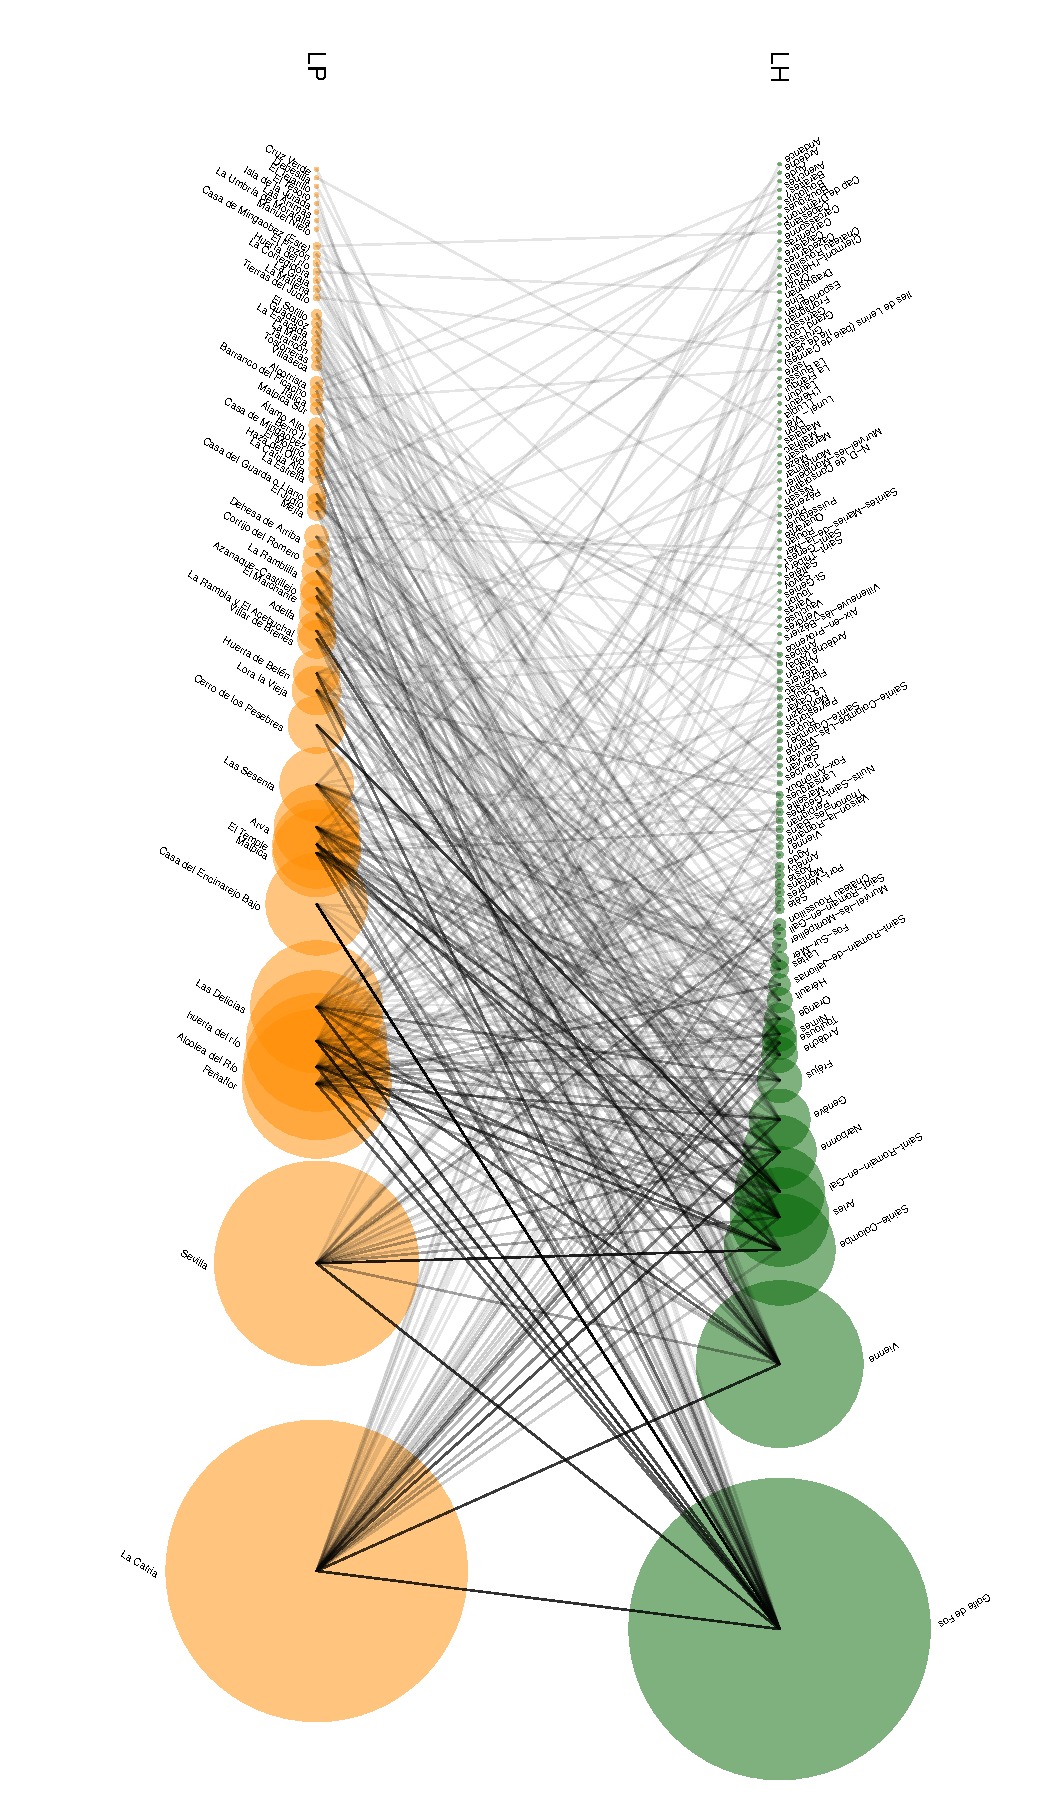
\includegraphics[height=3cm]{images/netrot.pdf}} \hfill
    \uncover<4->{\href{run:../../../../full_projects/icrates_abc/scripts/athens.mpg?onclick&loop}{\includegraphics[height=3cm]{../../../../full_projects/icrates_abc/scripts/testblack/map_athens_001.png}} }


    \uncover<5->{$\rightarrow$ Historians and Archaeologists building hypotheses and theories.}
\end{frame}

\begin{frame}
    Example of the economy (from Brughmans and Poblome 2016):
    \begin{center}
        \uncover<+->{
\includegraphics[height=3cm]{images/bang.jpg}} \hfil
        \uncover<+->{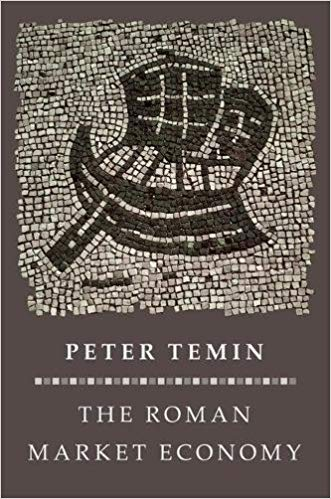
\includegraphics[height=3cm]{images/temin.jpg}} 
    \end{center}

    \uncover<+->{
        \begin{itemize}
            \item No general theories
            \item No common framework
            \item \dots
        \end{itemize}
        How to compare, quantify, test those theories?
    }
\end{frame}

\begin{frame}{Theoretical Framework}
Change in past society: \\
\uncover<+->{
\begin{center}
    Succession of social interactions.
\end{center}
}
    \vfil
    \begin{itemize}
        \item<+-> Highly stochastic,
        \item<+-> contingent,
        \item<+-> \ldots
    \end{itemize}
    \vfil
    \uncover<+->{ Not so far from problems encountered by Evolutionary Biology}

    \uncover<+->{Cultural evolution as an evolutionary process}
\end{frame}

\section{Cultural Evolution}
\begin{frame}{Evolutionary Process}
    Social Traits:
    \begin{center}
	\begin{table}
	    \center
	    \begin{tabular}{ccc}
		\uncover<2->{\includegraphics[height=3cm]{images/m80}} &
		\uncover<3->{\includegraphics[height=3cm]{images/m90}} &
		\uncover<4->{\includegraphics[height=3cm]{images/m10}} \\
		\uncover<2->{80's} & \uncover<3->{90's} & \uncover<4->{now}
	    \end{tabular}
	\end{table}
    \end{center}
    \uncover<5->{
            Same way biologist study frequencies of biological traits to understand past biological phenomena, we can use frequencies of cultural traits to understand past social changes.
}

\end{frame}


\begin{frame}{Cultural Evolution}
    \begin{itemize}
	\item<5->{ Culturally transmitted, socially learnt}
	\item<6->{ Different probabilities of transmission (differential reproduction $\rightarrow$ bias) }
    \end{itemize}
	\begin{center}
		\uncover<4->{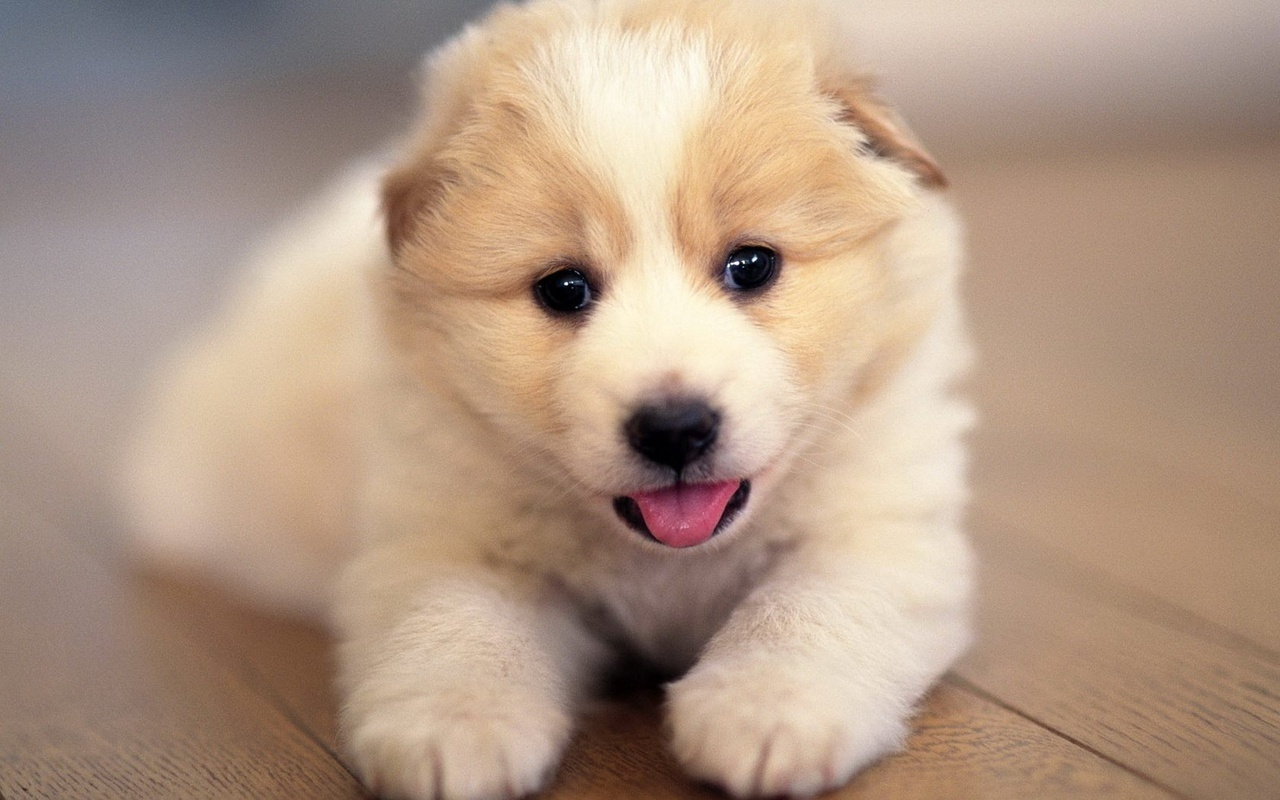
\includegraphics[width=3cm]{images/cutdog}}\\
		\vspace{.5cm}
		\uncover<2->{\includegraphics[width=2.5cm]{images/cutbaby}}
	    \hspace{1cm}
	    \uncover<3->{ \includegraphics[width=2cm]{images/pottery}}
	\end{center}
    \uncover<7>{$\rightarrow$ What mechanism drive the evolution of such traits?\\
    \invisible<1->{$\rightarrow$ What mechanism }generate such pattern?}
\end{frame}

\begin{frame}{What Generate Those Cultural changes?}
	Simple mechanisms (Bentley et al, 2004):
	\begin{itemize}
		\item<2->Random Copy 
		\item<3-> Frequency biased (conformist/anti-conformist\dots)
		\item<4->\dots	
	\end{itemize}
    \uncover<5->{Simple models, could be represented with equations and solved.}
	\uncover<2>{\begin{figure}
		\begin{columns}
			\begin{column}{.8\textwidth}
				\centering
				\includegraphics[width=.6\textwidth]{images/powerlawrepartition.jpg}
			\end{column}
			\begin{column}{.3\textwidth}
				\tiny
				Square: male names\\
				Circle: female names\\
				Dotted and plain lines: model result with different copy probabilities.\\
			From Bentley et al,~2004.
			\end{column}
		\end{columns}
	    \end{figure}}
\end{frame}

\begin{frame}
	\begin{center}
	    What if such mechanisms act on traits linked to economics?
	\end{center}
\end{frame}

\begin{frame}{A social traits an economic weight}
	\begin{center}
	    \only<1>{\includegraphics[width=.8\textwidth]{images/boubou1.png}}
	    \only<2>{\includegraphics[width=.8\textwidth]{images/boubou2.png}}
	    \only<3>{\includegraphics[width=.8\textwidth]{images/boubou3.png}}
	\end{center}
\end{frame}

\begin{frame}{Co-evolution of Economy and Culture}

    \vspace{2cm}
    \begin{center}
	\begin{overlayarea}{\textwidth}{\textheight}
	    \only<1>{\includegraphics[width=\textwidth]{images/map1.png}}
	    \only<2>{\includegraphics[width=\textwidth]{images/map2.png}}
	    \only<3>{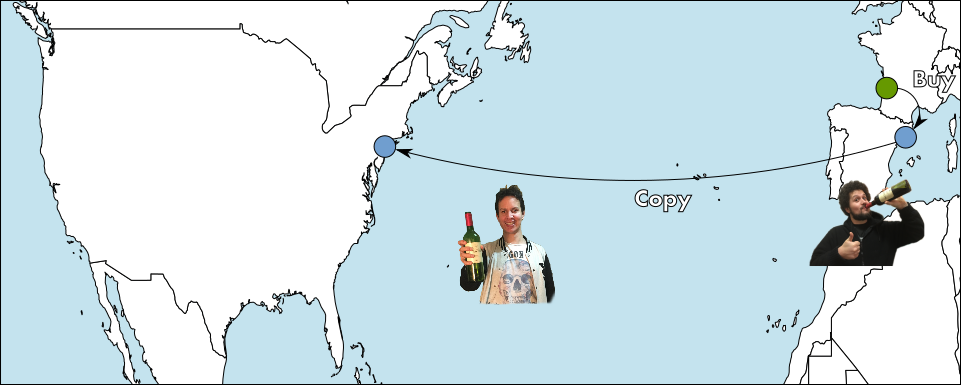
\includegraphics[width=\textwidth]{images/map3.png}}
	    \only<4>{\includegraphics[width=\textwidth]{images/map4.png}}
	    \only<5>{\includegraphics[width=\textwidth]{images/map5.png}}
	    \only<6>{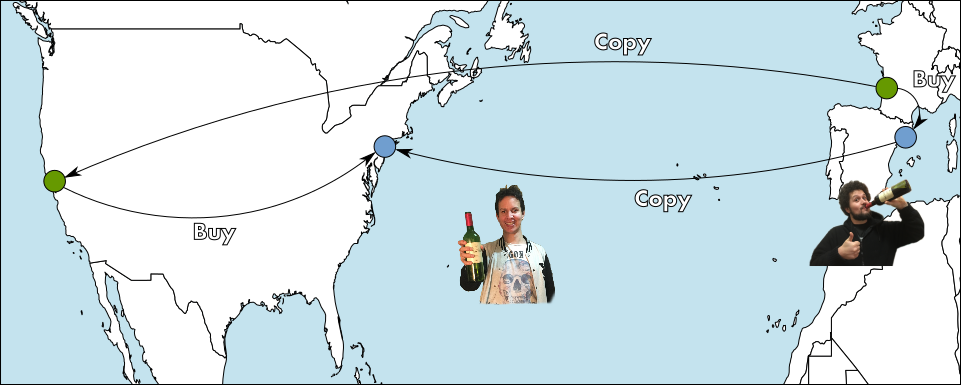
\includegraphics[width=\textwidth]{images/map6.png}}
	    \only<7>{\includegraphics[width=\textwidth]{images/map7.png}}
	    \only<8>{\includegraphics[width=\textwidth]{images/map8.png}}
	    \only<9>{\includegraphics[width=\textwidth]{images/map9.png}}
	    \only<10>{\includegraphics[width=\textwidth]{images/map10.png}}
	    \only<11>{\includegraphics[width=\textwidth]{images/graph1.png}}
	    \only<12>{\includegraphics[width=\textwidth]{images/graph2.png}}
	    \only<13>{\includegraphics[width=\textwidth]{images/graph3.png}}
	\end{overlayarea}

    \end{center}
\end{frame}


\section{ABM Framework}


\begin{frame}{General Modeling Framework}
    \begin{center}
	\includegraphics[width=.8\textwidth]{images/cooev.png}	
    \end{center}
    \uncover<2->{Equations?}
\end{frame}

\begin{frame}{General Modeling Framework}
    \vfill
    Agent Based Model:
    A general framework where we can implement hypothesis and theories.
    \begin{center}
	\includegraphics[width=.5\textwidth]{images/cooev.png}	
    \end{center}
    \vfill
	\begin{itemize}
	\item Different Cultural Mechanisms
    \vfill
	\item Different Trade Assumption
    \vfill
	\item Historical and Archaeological Evidences 
    \vfill
	\item Network Constraints
    \vfill
	\item \dots
    \vfill
	\end{itemize}
\end{frame}
	
\begin{frame}{Limitations}
    \begin{center}
	\includegraphics[width=.6\textwidth]{images/cooev.png}	
    \end{center}
    At each level, every action can be very costly:
    \begin{itemize}
        \uncover<2->{ \item  agents meet every other producers ($N^{2}\times(N_{goods}-1)$)}
        \uncover<3->{ \item  agents check what they have \& they need ($N_{good} \times 2$)}
        \uncover<4->{ \item  ranking of everyone ($N\times log(N)$}
        \uncover<5->{ \item  Social Learning (probabilistic copy ($N \times (Q)$ ($Q < N -1$) )}
        \uncover<6->{ \item  \dots }
    \end{itemize}
    \uncover<7->{$\rightarrow$ Need for parallelisation \huge}
\end{frame}


\begin{frame}{Pandora}
    Split space in different sub part run on different node communicating through MPI.
    \begin{figure}[h]
        \centering
        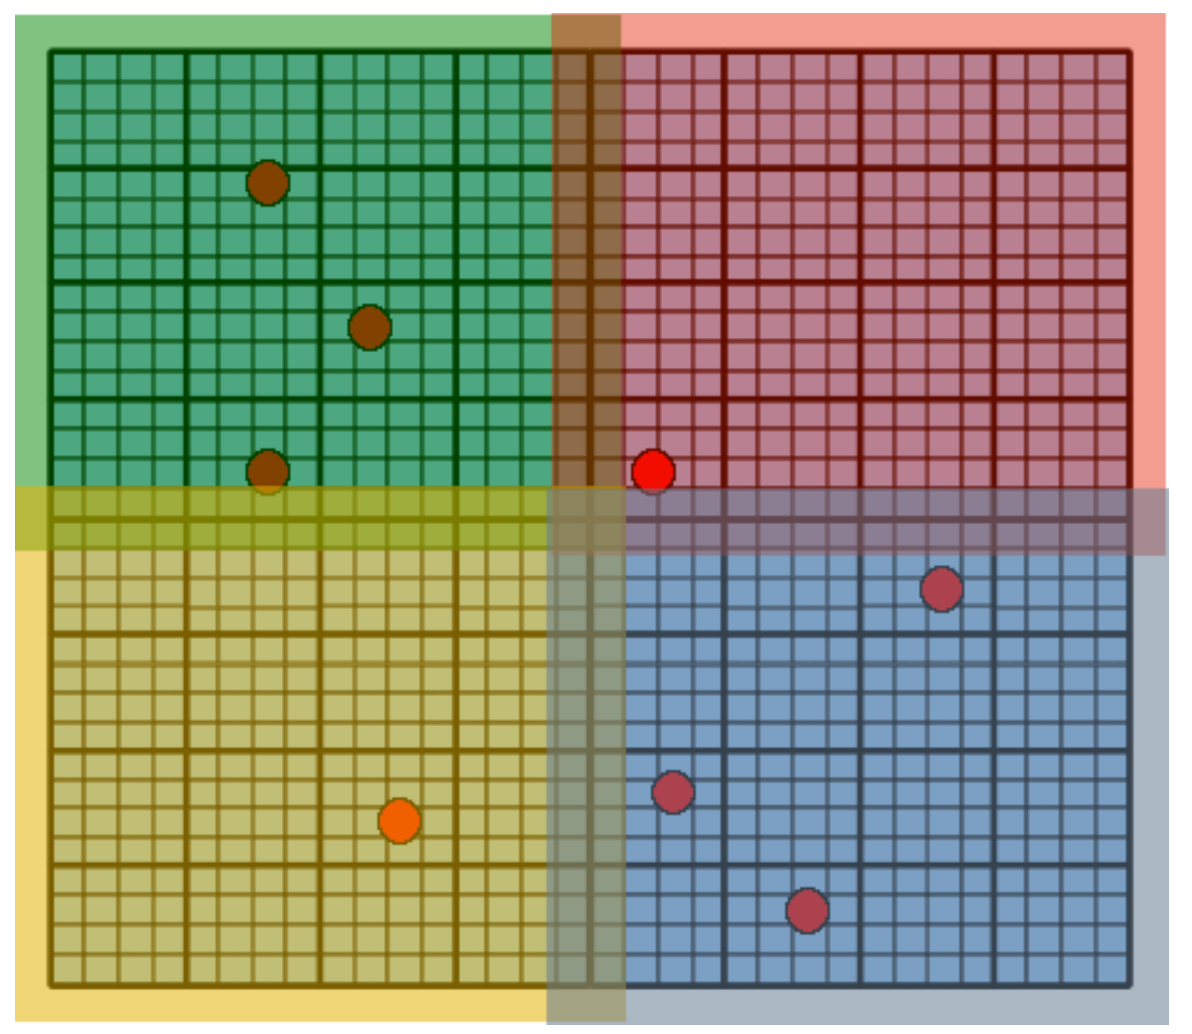
\includegraphics[width=.3\textwidth]{images/splitPandora.png}
        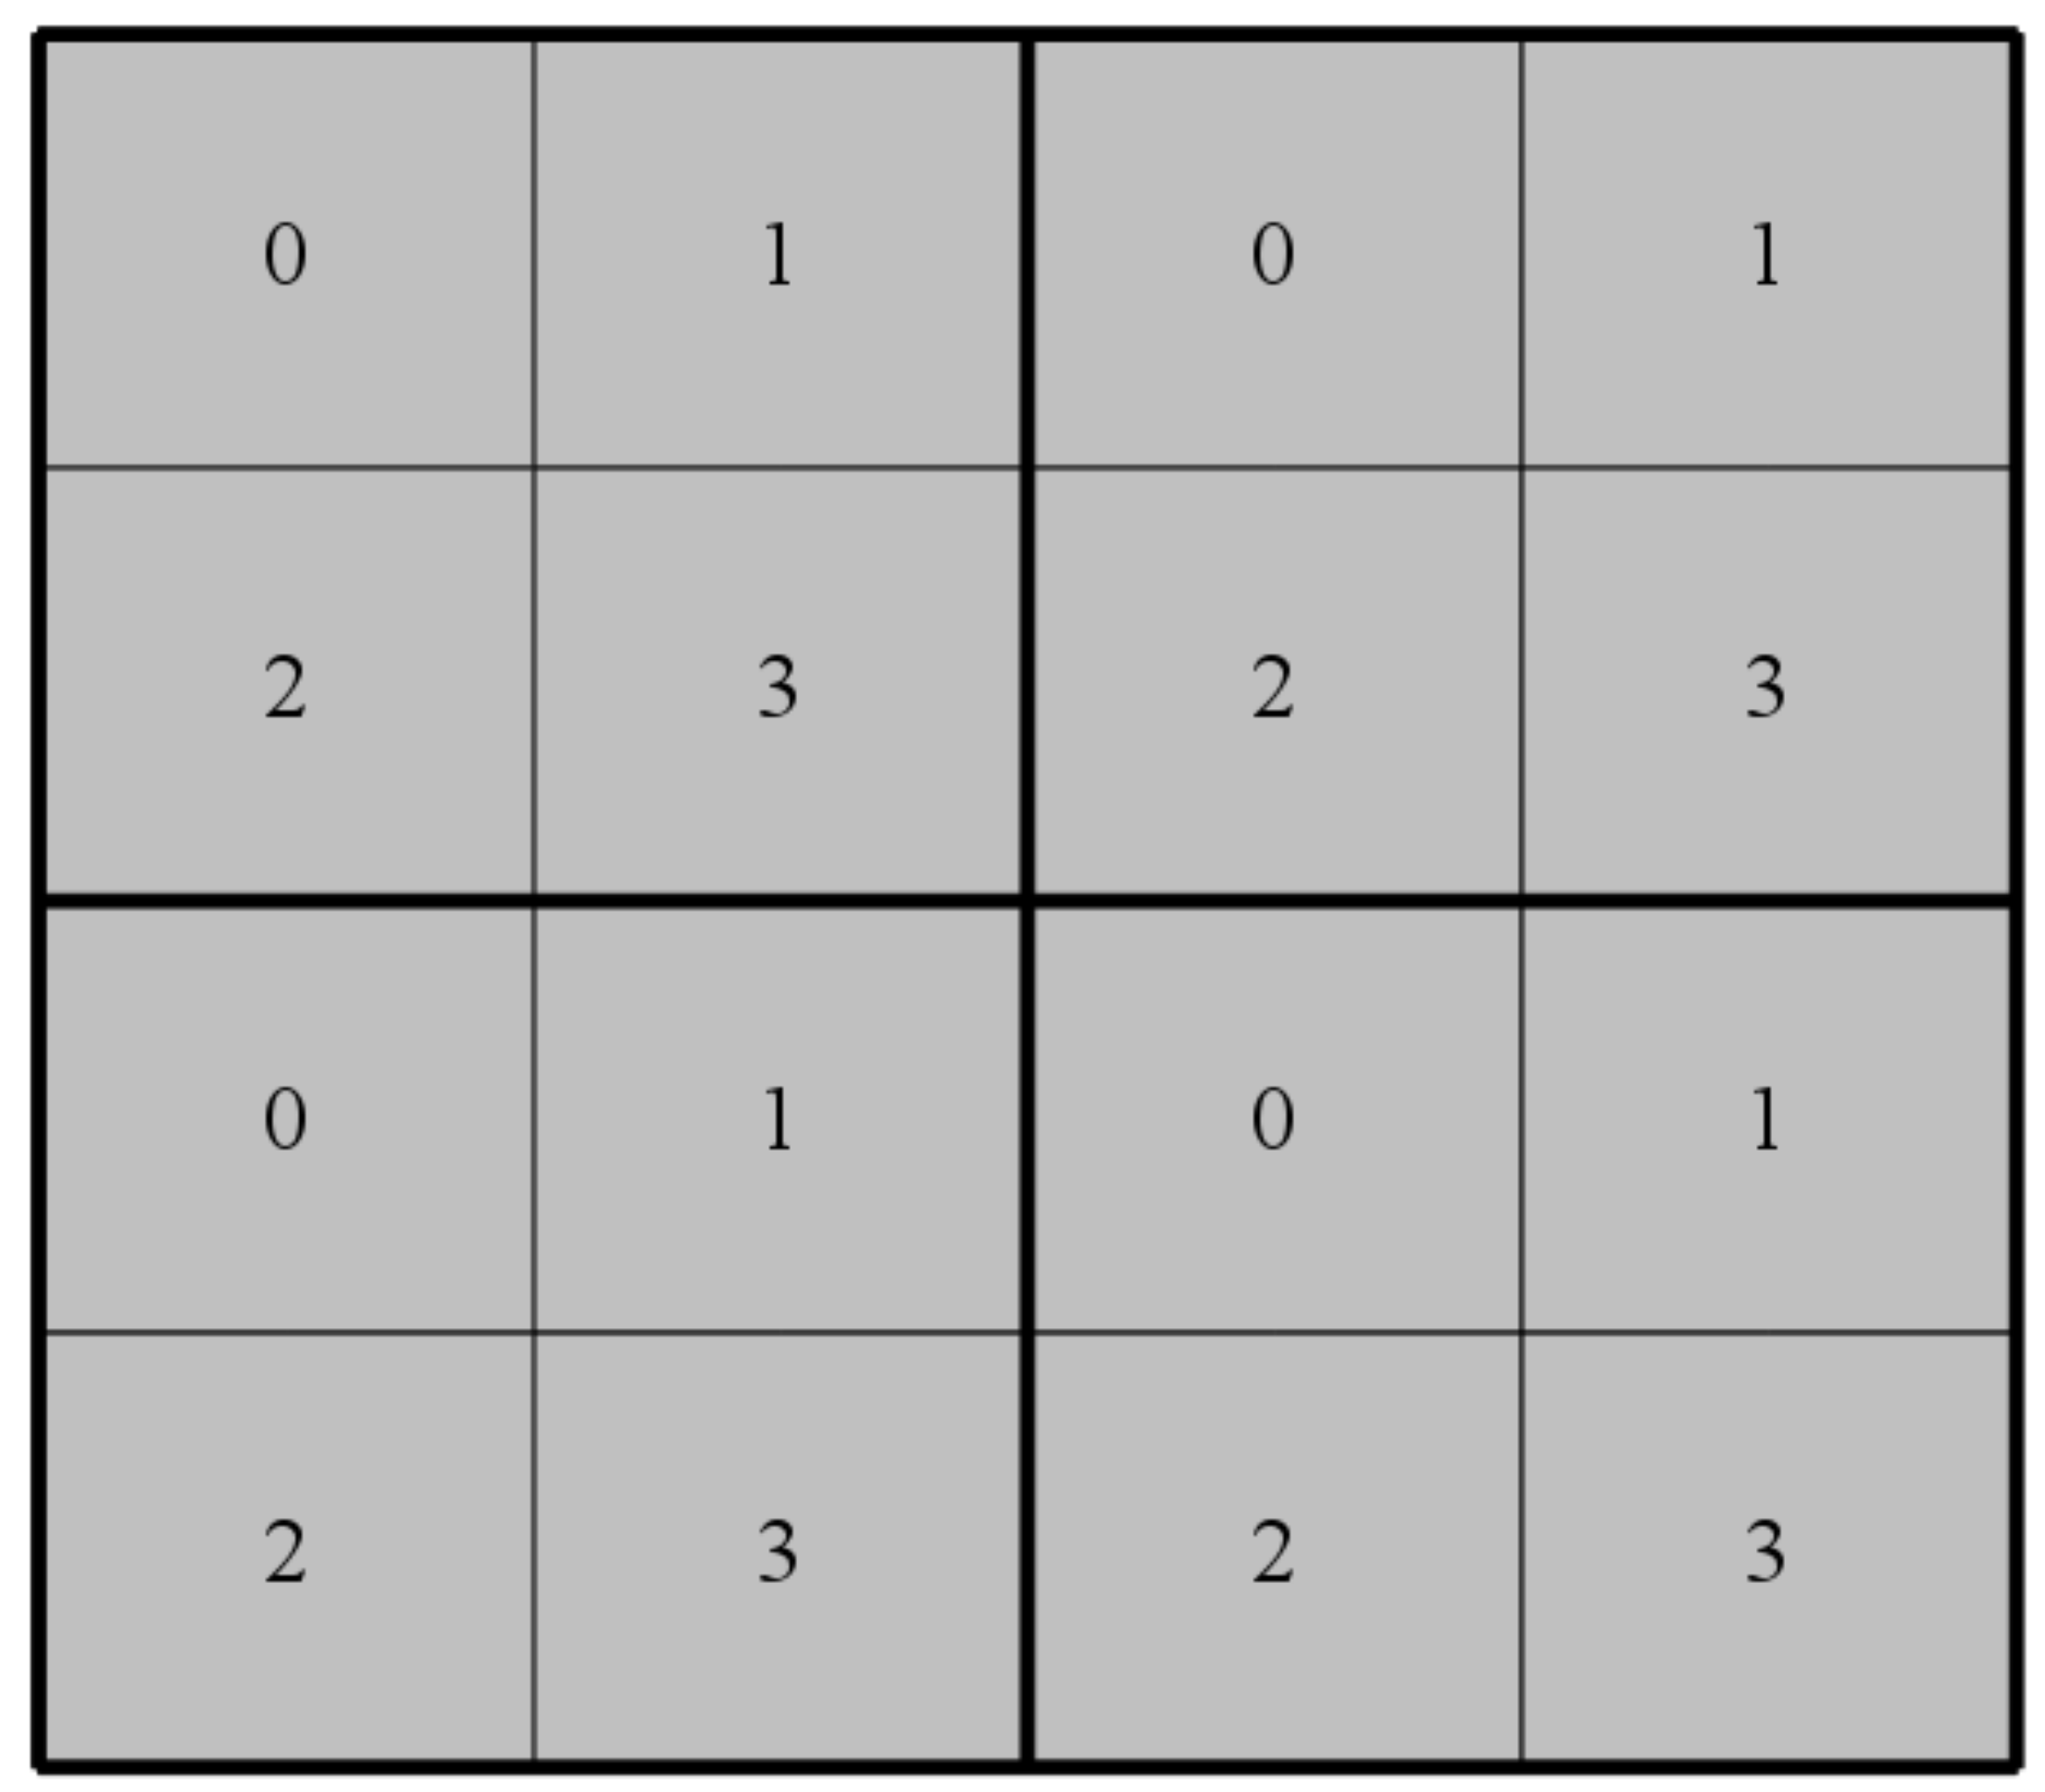
\includegraphics[width=.3\textwidth]{images/numbersCPU.png}
        \caption{Repartition of agents between nodes. from Rubio-Campillo 2012.}
        \label{fig:splp}
    \end{figure}
\end{frame}

\begin{frame}{Results: Economic Dynamics}
    Carrignon, Montanier \& Rubio-Campillo 2015, in line with Gintis 2006:
	\begin{figure}
	    \caption{Example for 3 goods and 500 agents}
	    \begin{columns}
		\column{.5\textwidth}
		\includegraphics[height=\textwidth]{images/ClearingPriceDistanceEvolutionForTrade-G3N500.pdf}\\
	    \end{columns}
		@~Equilibrium: personal values  $\rightarrow$ optimal (shared) values.
	\end{figure}
\end{frame}

\begin{frame}
    Now we have a model. How can we use it to learn about:\\
    The Economy of the Roman Empire (work in collaboration with Iza Romanowska \& Tom Brughmans).

		\includegraphics[height=3cm]{images/fortGreekPlaceAndAmphora} \hfill
		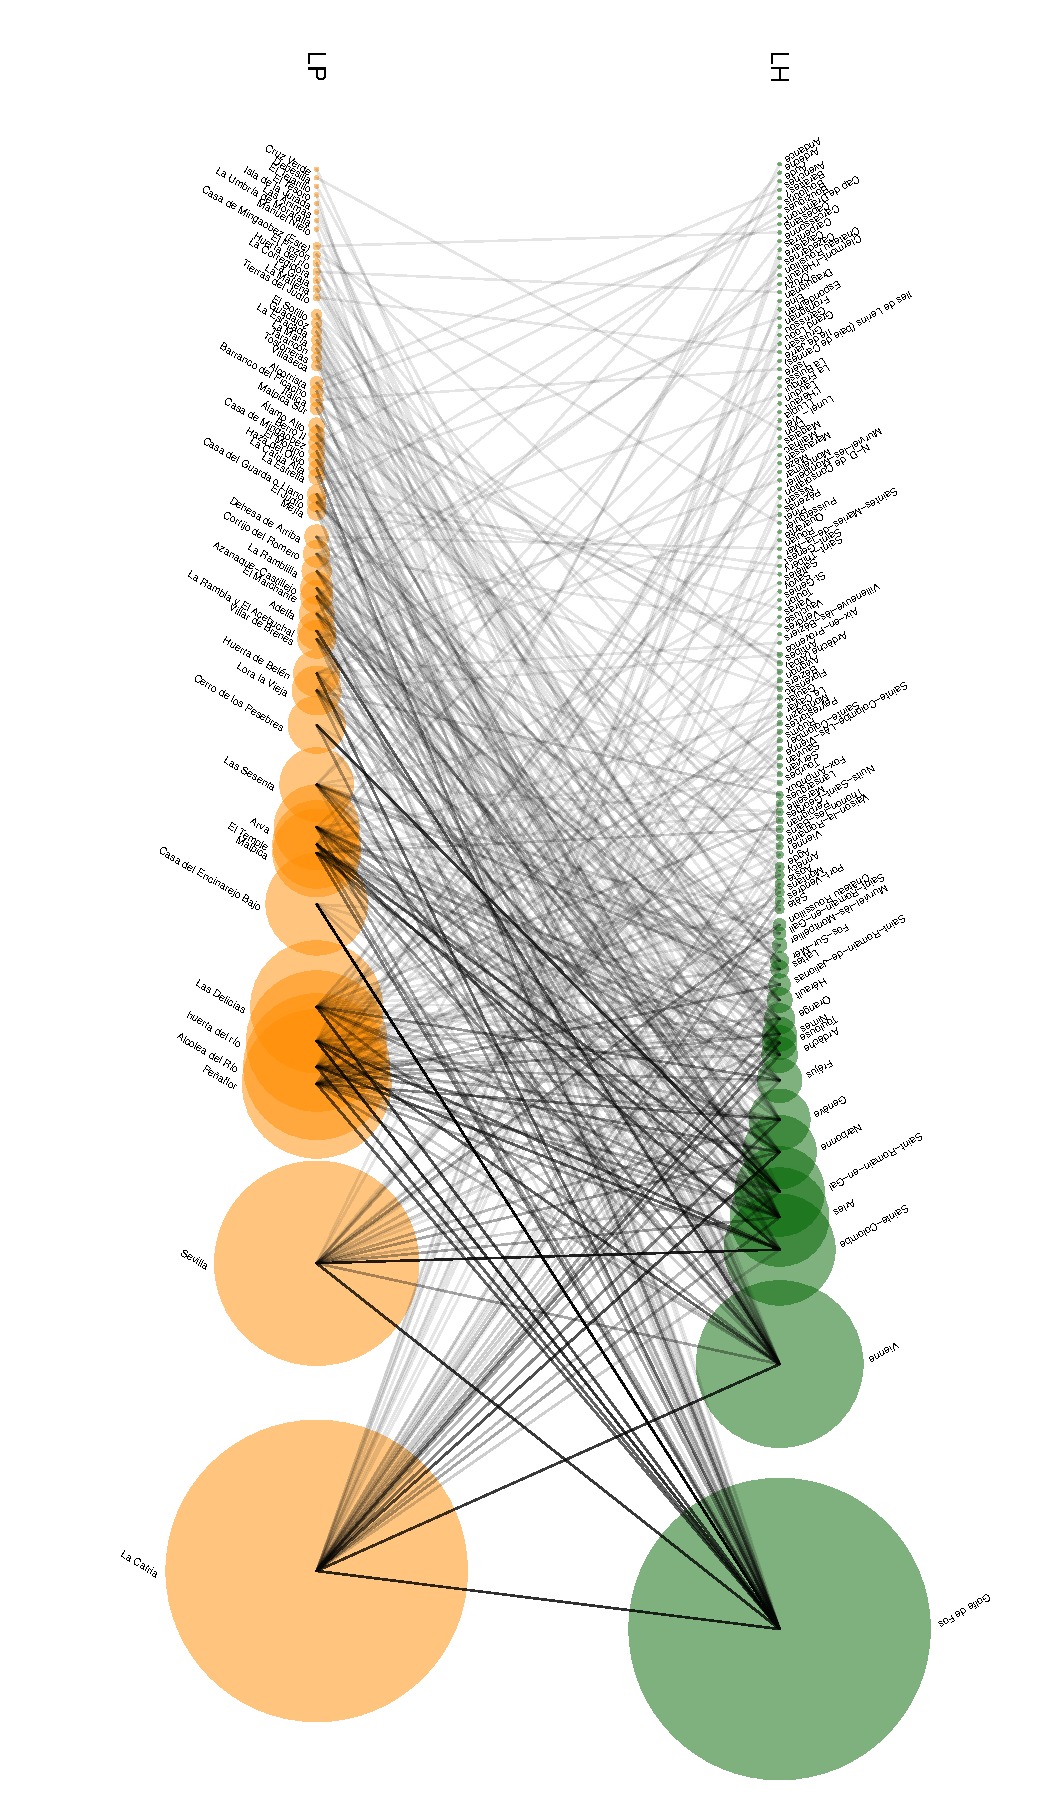
\includegraphics[height=3cm]{images/netrot.pdf} \hfill
        \href{run:../../../../full_projects/icrates_abc/scripts/athens.mpg?onclick&loop}{\includegraphics[height=3cm]{../../../../full_projects/icrates_abc/scripts/testblack/map_athens_001.png}} 

    \begin{itemize}
        \item Model with lot of parameters and few a priori knowledge of impact of those parameters,  
        \item  Incomplete, biased, small dataset
    \end{itemize}
    
\end{frame}

\section{Bayesian Inference}

\begin{frame}{Bayesian Inference:}
    $$P(A|B)=\frac{P(B|A)*P(A)}{P(B)}$$
        \begin{center}
            \large
            What is the probability of something knowing something else?
        \end{center}
      $A$ can be a model with parameters ($\theta$) and $B$ our evidence (E), the posterior becomes: 
      $$P(\theta|E)$$

      \begin{itemize}
          \item Test the ability of model to explain the data
          \item Compare different model against same data set
          \item \ldots
      \end{itemize}

\end{frame}

\begin{frame}{Problem}
    When you cannot calculate all probabilities, simulate the model.
    \begin{center}
        Approximate Bayesian Computation (Beaumont 2002)\\
        (and its flavors)
    \end{center}
    $\rightarrow$ After simulations, only the parameter that produces output close enough to the data ($<\epsilon$) are selected to draw the posterior.
\end{frame}

%\begin{frame}{}
%        \textcolor{tracblue}{\large How to know more about something?}
%        \vspace{1cm}
%    \begin{columns}
%
%        \begin{column}{0.6\linewidth}
%            \visible<2->{Claude Bernard style:}
%            \begin{itemize}
%                \item<3-> Cut in pieces
%                \item<4-> Do something
%                \item<5-> Repeat
%            \end{itemize}
%            \visible<6->{Einstein style:}
%
%            \begin{itemize}
%                \item<7-> Theories \& laws + Logic \& Maths = New  Theories, new laws, new predictions.
%                \item<8-> Wait until someone observe something inline with your predictions 
%            \end{itemize}
%
%
%        \end{column}
%        \begin{column}{0.3\linewidth}
%
%            \only<2-5>
%            {
%                \begin{figure}[h]
%                    \centering
%                    \includegraphics[width=.5\textwidth]{images/cloclobeber.png}\\
%                    {\tiny From: collection BIU Santé Médecine}
%                \end{figure}
%            }
%            \only<6->
%            {
%                \begin{figure}[h]
%                    \centering
%                    \fbox{\parbox{\textwidth}{\small images/any-image-with-the-face-of-einstein-choose-the-one-you-prefer.png}}
%                    {\tiny From: somewhere in your prefrontal cortex}
%                \end{figure}
%            }
%
%
%        \end{column}
%
%    \end{columns}
%
%\end{frame}
%
%\begin{frame}{What if\ldots}
%    \begin{itemize}
%        \item<+-> Not possible to cut anything.
%        \item<+-> No formal theorie nor laws about the studied object.
%    \end{itemize}
%        \pause
%    \begin{figure}[h]
%        \centering
%        \includegraphics[height=.3\textheight]{images/ghost.jpg}\hfill
%        \pause
%        \includegraphics[height=.3\textheight]{images/hollow_man_towel.jpg}
%    \end{figure}
%\end{frame}
%
%
%\begin{frame}{}
%    How to get more informations ?
%    \begin{figure}
%        \includegraphics[height=.3\textheight]{images/ghost.jpg}\hfill
%        \includegraphics[height=.3\textheight]{images/hollow_man_towel.jpg}\\
%        \visible<2->{\includegraphics[height=.3\textheight]{images/hollow_man_water.jpg}} \hfill
%        \visible<3>{\includegraphics[height=.3\textheight]{images/ghostbusters.jpg}}
%    \end{figure}
%
%\end{frame}


%\begin{frame}{}
%    \center
%    Approximate Baeysian Computation\\Linking model and data for an experimental approach to theory.\\
%    \vspace{1cm}
%    \visible<2->{AKA}\\
%    \vspace{1cm}
%    \visible<3->{{\huge \bf \textcolor{tracblue}{The Cool Hunters of the Unknown }}}
%\end{frame}


%\begin{frame}{Hypothetical case}
%    \begin{figure}
%        \includegraphics[height=.8\textheight]{images/sagregang/empty.jpg}
%    \end{figure}
%\end{frame}
%
%\begin{frame}{Limitations}
%    \begin{itemize}
%        \item<+-> This is not moving
%        \item<+-> Impossible to touch or manipulate\ldots
%        \item<+-> Some shape can be luckily gathered 
%    \end{itemize}
%    \vfil
%    \begin{figure}
%        \visible<+->{\includegraphics[height=.3\textheight]{images/hollow_man_waterNo.jpg} \hfill}
%        \visible<+->{\includegraphics[height=.3\textheight]{images/ghostbustersNo.jpg}}
%    \end{figure}
%\end{frame}
%
%\begin{frame}{Material \& Methods}
%    \begin{figure}
%        \pause
%        \includegraphics[height=.4\textheight]{images/huntersTools.jpg} \\
%        \vfill
%        \pause
%        \includegraphics[width=.4\textwidth]{images/huntersWaiting.jpg} \hfill
%        \pause
%        \includegraphics[width=.4\textwidth]{images/huntersThrowing.jpg} 
%    \end{figure}
%\end{frame}
%
%\begin{frame}{Data Gathering \& Data Analysis}
%    \begin{figure}
%        \only<1>{\includegraphics[height=.8\textheight]{images/sagregang/empty.jpg}}
%        \only<2>{
%            Throw and take a pictures\\
%            \includegraphics[width=.4\textwidth]{images/huntersWaiting.jpg} \hfill
%            \includegraphics[width=.4\textwidth]{images/huntersThrowing.jpg} 
%        }
%        \only<3>{\includegraphics[height=.8\textheight]{images/sagregang/shape.jpg}}
%        \only<4>{
%            Throw again and take a pictures\\
%            \includegraphics[width=.4\textwidth]{images/huntersWaiting.jpg} \hfill
%            \includegraphics[width=.4\textwidth]{images/huntersThrowing.jpg} 
%        }
%        \only<5>{\includegraphics[height=.8\textheight]{images/sagregang/reality_shape.jpg}}
%    \end{figure}
%\end{frame}

\begin{frame}{Modeling \& Simulation}
    \begin{figure}
        \includegraphics<+->[height=.8\textheight]{images/sagregang/reality_shape.jpg}
        \hfill
        \includegraphics<+>[height=.8\textheight]{images/sagregang/bare_model.jpg}
        \includegraphics<+>[height=.8\textheight]{images/sagregang/model_halfsimu.jpg}
        \includegraphics<+>[height=.8\textheight]{images/sagregang/model_adjusting.jpg}
        \includegraphics<+>[height=.8\textheight]{images/sagregang/model_fullsimuHigh.jpg}
        \includegraphics<+>[height=.8\textheight]{images/sagregang/model_halfsimuLow.jpg}
        \includegraphics<+>[height=.8\textheight]{images/sagregang/model_fullsimuLow.jpg}
        \includegraphics<+>[height=.8\textheight]{images/sagregang/model_adjustingB.jpg}
        \includegraphics<+>[height=.8\textheight]{images/sagregang/model_fullsimuLow+arm.jpg}
    \end{figure}
\end{frame}

\begin{frame}{Modeling \& Simulation}
    \begin{figure}
        \visible<2>{\includegraphics[height=.8\textheight]{images/sagregang/reality_shape+details.jpg}}
        \hfill
        \visible<1->{\includegraphics[height=.8\textheight]{images/sagregang/model_fullsimuLow+arm+details.jpg}}
    \end{figure}
\end{frame}


\begin{frame}{Evidences}
    The ICRATES database:
    \begin{itemize}
        \item 5 types of Sigilata used to produce tableware (bowl, cup, plates)
        \item 178 sites
        \item 500 years (200~BC--300~AD)
    \end{itemize}

    \begin{center}
        \href{run:../../../../full_projects/icrates_abc/scripts/athens.mpg?onclick&loop}{\includegraphics[height=2.5cm]{../../../../full_projects/icrates_abc/scripts/testblack/map_athens_001.png}} 
    \end{center}
    \visible<2->{
    \begin{table}
        \centering
        \begin{tabular}{cc}
            \includegraphics[width=0.38\textwidth]{images/realdistrib100-b.png} &
            \includegraphics[width=0.38\textwidth]{images/realdivers100-b.png} \\
            Diversity within sites & Distributions among sites 
        \end{tabular}
    \end{table}
}
\end{frame}

\begin{frame}{The Model}
    \begin{figure}[h]
        \centering
        \includegraphics[width=.5\textwidth]{images/cooev.png}
    \end{figure}
    Agent based model  presented before with dynamic processes interacting:
    \begin{itemize}
        \item Cultural activity (people can learn from each other)
        \item Economic activity (people can trade with each other)
    \end{itemize}
    + one flavor of ABC: Sequential Monte Carlo Sampling:
    \begin{itemize}
        \item The acceptance level is adjusted during the simulation.
    \end{itemize}
\end{frame}

\begin{frame}{Sequential ABC}

    One simulation

    \vspace{20pt}

    \only<1>{\href{run:presentation_script/video_one_simulation_good/output.mpg?autostart&noloop}{\includegraphics[width=0.9\textwidth]{presentation_script/video_one_simulation_good/one_sim_ex_step-002.png}}}
    \only<2>{\includegraphics[width=0.9\textwidth]{presentation_script/video_one_simulation_good/one_sim_ex_step-comp.png}}
    \only<3>{\includegraphics[width=0.9\textwidth]{presentation_script/video_one_simulation_good/one_sim_ex_step-score.png}}
    \only<4>{\includegraphics[width=0.9\textwidth]{presentation_script/video_one_simulation_good/one_sim_ex_step-check.png}}
    \only<5>{\includegraphics[width=0.9\textwidth]{presentation_script/video_one_simulation_good/one_sim_ex_step-update.png}}
\end{frame}


\begin{frame}{Sequential ABC}


    An do the same with another simulation %Change good with good1 and bad i

    \vspace{20pt}
    \only<1>{\href{run:presentation_script/video_one_simulation_good2/output.mpg?autostart&noloop}{\includegraphics[width=0.9\textwidth]{presentation_script/video_one_simulation_good2/one_sim_ex_step-002.png}}}
    \only<2>{\includegraphics[width=0.9\textwidth]{presentation_script/video_one_simulation_good2/one_sim_ex_step-comp.png}}
    \only<3>{\includegraphics[width=0.9\textwidth]{presentation_script/video_one_simulation_good2/one_sim_ex_step-score.png}}
    \only<4>{\includegraphics[width=0.9\textwidth]{presentation_script/video_one_simulation_good2/one_sim_ex_step-check.png}}
    \only<5>{\includegraphics[width=0.9\textwidth]{presentation_script/video_one_simulation_good2/one_sim_ex_step-update.png}}

\end{frame}


\begin{frame}{Sequential ABC}


    And another\ldots %Change good with good1 and bad i

    \vspace{20pt}
    \only<1>{\href{run:presentation_script/video_one_simulation_good3/output.mpg?autostart&noloop}{\includegraphics[width=0.9\textwidth]{presentation_script/video_one_simulation_good3/one_sim_ex_step-002.png}}}
    \only<2>{\includegraphics[width=0.9\textwidth]{presentation_script/video_one_simulation_good3/one_sim_ex_step-comp.png}}
    \only<3>{\includegraphics[width=0.9\textwidth]{presentation_script/video_one_simulation_good3/one_sim_ex_step-score.png}}
    \only<4>{\includegraphics[width=0.9\textwidth]{presentation_script/video_one_simulation_good3/one_sim_ex_step-check.png}}
    \only<5>{\includegraphics[width=0.9\textwidth]{presentation_script/video_one_simulation_good3/one_sim_ex_step-update.png}}

\end{frame}

\begin{frame}{Sequential ABC}
    Until you have enough
    \vspace{20pt}
    \only<1>{ \href{run:presentation_script/full_video_epsilon_0.15/output1.mpg?autostart&noloop}{\includegraphics[width=0.9\textwidth]{presentation_script/full_video_epsilon_0.15/all_sim_frame-00094.png}}  }
    \only<2>{ \href{run:presentation_script/full_video_epsilon_0.15/output2.mpg?autostart&noloop}{\includegraphics[width=0.9\textwidth]{presentation_script/full_video_epsilon_0.15/all_sim_frame-00640.png}}  }
\end{frame}

\begin{frame}
    And repeat the same but being more restrictive:
    \vspace{20pt}
    \only<1>{ \href{run:presentation_script/full_video_epsilon_0.012/output1.mpg?autostart&noloop}{\includegraphics[width=0.9\textwidth]{presentation_script/full_video_epsilon_0.15/all_sim_frame-00094.png}}  }
    \only<2>{ \href{run:presentation_script/full_video_epsilon_0.012/output2.mpg?autostart&noloop}{\includegraphics[width=0.9\textwidth]{presentation_script/full_video_epsilon_0.15/all_sim_frame-00640.png}}  }

\end{frame}

\begin{frame}
    \centering
    \includegraphics[height=0.95\textheight]{images/result_abc_rand.png}
\end{frame}

\begin{frame}{Hypothesis Testing}
    Compare two different hypothesis on the social learning mechanism:
    \begin{itemize}
        \item Copy the bests $\rightarrow$ Random copy 
    \end{itemize}
\end{frame}


\begin{frame}{Hypothesis Testing}

    Compare number of simulation needed to reach the more restrictive epsilons:
    \begin{itemize}
        \item $564\,211$~simulations: unbiased social learning mechanism 
        \item $209\,395$~success-biased: social learning mechanism. 
    \end{itemize}
    \begin{figure}
        \includegraphics[width=.4\textwidth]{images/curve_ratio.png}
    \end{figure}
\end{frame}

\begin{frame}{Compare parameters}
    \begin{figure}[!ht]
        \centering
        \includegraphics[width=.4\textwidth]{images/random_vs_bestbias.png}
        \caption{Posterior distribution for all parameters}
    \end{figure}

    \subsubsection{Rate of Social Learning} the probability that at each time step someone copy the strategies of someone else
    \input{tables/hdr_copy.tex}
    \begin{figure}[!ht]
        \centering
        \includegraphics[width=.4\textwidth]{images/densities_copy.png}
        \caption{Posterior distribution for the Rate of Social Learning}
        \label{fig:copy}
    \end{figure}
\end{frame}


\begin{frame}{ABC summary}
    Approximate Bayesian Computation allows to link data to models by giving us the probability of one model to reproduce observed patterns.
    \begin{itemize}
        \item<+-> Flexible,
        \item<+-> Few assumptions needed (neither on data nor model side),
        \item<+-> Heavy computational cost,
        \item<+-> Central role of transdisciplinarity (central role interpretation and expert knowledge). No strict answer ($<.05 \rightarrow$ OK,$>.05 \rightarrow$ not OK).
    \end{itemize}
 
\end{frame}

\section{Conclusion}

\begin{frame}{General Conclusion}
    Status of simulation and computer model vs empirical research:
    \begin{itemize}
        \item Opaque Thought Experiment (Di Paolo, Noble and Bullock)experience on it's own
        \item Hybrid status in-between experiment and theories.
    \end{itemize}

    \vspace{1cm}

    \textcolor{tracblue}{New ways to know more about something, closer to experimental approach}
    \begin{columns}
        \begin{column}{0.6\linewidth}
            \visible<2->{Claude Bernard style:}
            \begin{itemize}
                \item<3-> Cut in pieces
                \item<4-> Do something under some condition
                \item<5-> Repeat with other conditions
                \item<6-> Conclusion
            \end{itemize}
        \end{column}
        \begin{column}{0.3\linewidth}

            \only<2-6>
            {
                \begin{figure}[h]
                    \centering
                    \includegraphics[width=.5\textwidth]{images/cloclobeber.png}\\
                    {\tiny From: collection BIU Santé Médecine}
                \end{figure}
            }
        \end{column}
    \end{columns}
\end{frame}

\begin{frame}{Limitations}
    \begin{itemize}
        \item<+-> High Technical Specialisation At every level
            \begin{itemize}
                \item <+-> Formulation of Hypotheses from actual Knowledge
                \item <+-> implementation (formalization)
                \item <+-> simulation
                \item <+-> analysis
            \end{itemize}
        \item<+-> Access to supercomputer 
        \item<+-> Ecological Cost
    \end{itemize}
    
\end{frame}


\begin{frame}
	\begin{center}
		\includegraphics[width=2cm]{images/LOGO-ERC.jpg} \hfil	\includegraphics[width=3cm]{images/epnetLogo.png}\\
		\includegraphics[width=3cm]{images/leverhulme}\\
		\vspace{.5cm}
		Thank you for you attention\\
		\vspace{.5cm}
		\scriptsize
			http://www.roman-ep.net/\\
			@simoncarrignon\\
		\vspace{.5cm}
		\includegraphics[width=4cm]{images/bscLogo}\\
	\end{center}
\end{frame}

\end{document}


